\documentclass[uplatex,dvipdfmx]{ujreport}

\author{片又佑美}
\title{ペンローズタイル張り上のライツアウトゲーム}

\usepackage{tikz,pgf,float}
\usepackage{amsmath}
\usepackage{amsfonts}

\begin{document}
\maketitle
\tableofcontents
\chapter{序}
\chapter{ペンローズタイル張り}
\section{ペンローズタイルの構成}
ペンローズタイル張りを構成するためには
次のような三角形の分割、拡大操作を繰り返す。
タイプAの三角形は二辺の長さが$1$でそれに
挟まれる角度が$\frac{\pi}{5}$の三角形である。
タイプAの三角形を$\tau$倍に拡大し、$\tau:1$に分割したものが図2.1である。

以下では黄金比$\tau$を以下のように定める。
\[
 \tau^2 = \tau + 1
\]
つまり、$\tau$は
\begin{equation}
 \tau =\frac{1+\sqrt{5}}{2}
\end{equation}
を満たす。


\begin{figure}[H]
  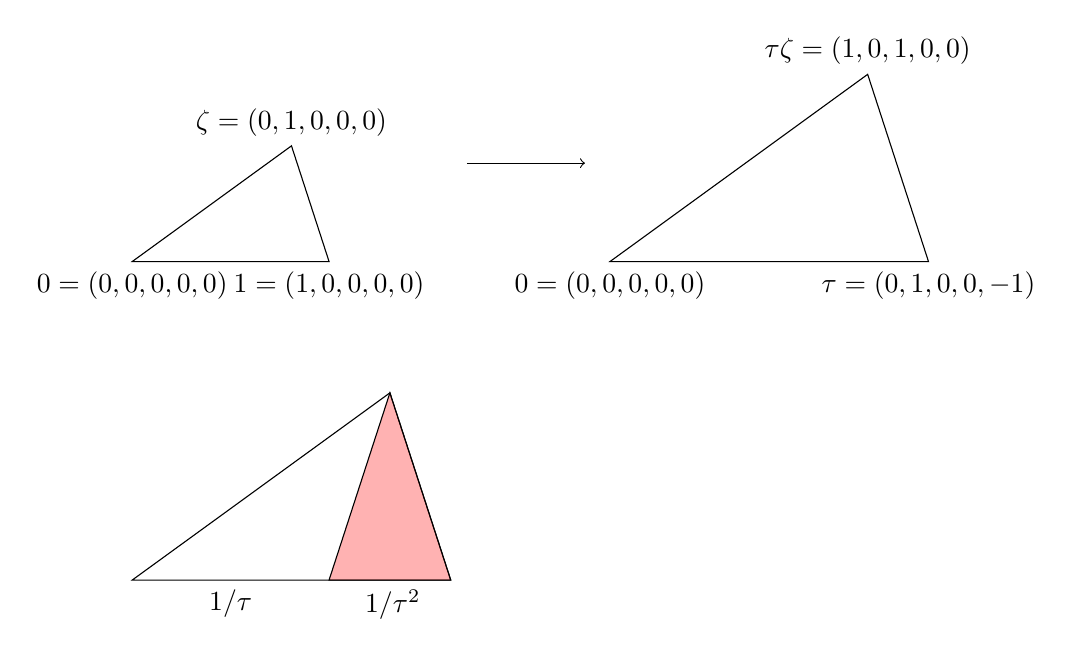
\begin{tikzpicture}[scale=2.5]
   \draw (0,0) -- (1,0) -- (36:1) -- cycle;
   \draw (0,0) node[below] {$0=(0,0,0,0,0)$};
   \draw (1,0) node[below] {$1=(1,0,0,0,0)$};
   \draw (36:1) node[above] {$\zeta=(0,1,0,0,0)$};
 
   \draw[->] (1.7,0.5)--(2.3,0.5);
   
   \begin{scope}[scale=(sqrt(5)+1)/2,xshift=1.5cm]
    \draw (0,0) -- (1,0) -- (36:1) -- cycle; 
    \draw (0,0) node[below] {$0=(0,0,0,0,0)$};
    \draw (1,0) node[below] {$\tau=(0,1,0,0,-1)$};
    \draw (36:1) node[above] {$\tau\zeta=(1,0,1,0,0)$};
   \end{scope}
   \begin{scope}[scale=(sqrt(5)+1)/2,yshift=-1cm]
    \draw (0,0) -- (1,0) -- (36:1) -- cycle; 
    \draw[fill=red,fill opacity=0.3] ({(sqrt(5)-1)/2},0) -- (36:1) --(1,0) -- cycle;
    \draw ({(sqrt(5)-1)/4},0) node[below] {$1/\tau$};
    \draw ({(sqrt(5)-1)/2+0.2},0) node[below] {$1/\tau^2$};
   \end{scope}
 \end{tikzpicture} 
\caption{タイプAの三角形の分割}
\end{figure}

そして、タイプBの三角形は二辺の長さが$1$でそれに
挟まれる角度が$\frac{3}{5}\pi$の三角形である。
タイプBの三角形を$\tau$倍に拡大し、$\tau:1$に分割したものが図2.2である。

\begin{figure}[H]
  \begin{tikzpicture}[scale=2.5]
   \draw (0,0) -- (1,0) -- (36:{(sqrt(5)+1)/2}) -- cycle;
   \draw (0,0) node[below] {$0=(0,0,0,0,0)$};
   \draw (1,0) node[below] {$1=(1,0,0,0,0)$};
   \draw (36:{(sqrt(5)+1)/2}) node[above] {$\tau\zeta=(1,0,1,0,0)$};
 
   \draw[->] (1.7,0.5)--(2.3,0.5);
   
   \begin{scope}[scale=(sqrt(5)+1)/2,xshift=1.5cm]
    \draw (0,0) -- (1,0) -- (36:{(sqrt(5)+1)/2}) -- cycle; 
    \draw (0,0) node[below] {$0=(0,0,0,0,0)$};
    \draw (1,0) node[below] {$\tau=(0,1,0,0,-1)$};
    \draw (36:{(sqrt(5)+1)/2}) node[above] {$\tau^2\zeta=(0,2,0,1,-1)$};
   \end{scope}
   \begin{scope}[scale=(sqrt(5)+1)/2,yshift=-1.2cm]
    \draw (0,0) -- (1,0) -- (36:{(sqrt(5)+1)/2}) -- cycle; 
    \draw ({(sqrt(5)-1)/2},0) -- (36:1) --(1,0) -- cycle;
    \draw ({(sqrt(5)-1)/4},0) node[below] {$1/\tau$};
    \draw ({(sqrt(5)-1)/2+0.2},0) node[below] {$1/\tau^2$};
   \end{scope}
 \end{tikzpicture} 
\caption{タイプBの三角形の分割}
\end{figure}

平面$\mathbb{R}^2$を複素平面$\mathbb{C}^2$とみなすことで拡大や細文、回転といった操作を複素数同士の掛け算や足し算によって表現できる。
\[
  \zeta =\cos \frac{\pi}{5}+\sin \frac{\pi}{5}
\]
と定める。この時、関係式
\[
  \zeta^5 =-1, \zeta^{-1}=-\zeta^4
\]
$\tau$と$\zeta$の関係式
\[
  \tau =\zeta+\zeta^{-1}
\]
が成り立つ。従って
\begin{equation}
  \frac{1}{\tau} =\tau-1=\zeta+\zeta^{-1}-1
\end{equation}

が成り立つ。

ペンローズタイル張りに現れるタイルの頂点の座標は整数$5$個からなるベクトル$x=(x_0,x_1,x_2,x_3,x_4)$を用いて
\begin{equation}
 x_0+x_1\zeta+x_2\zeta^2+x_3\zeta^3+x_4\zeta^4
\end{equation}
と表現できる。

\begin{figure}[H]
 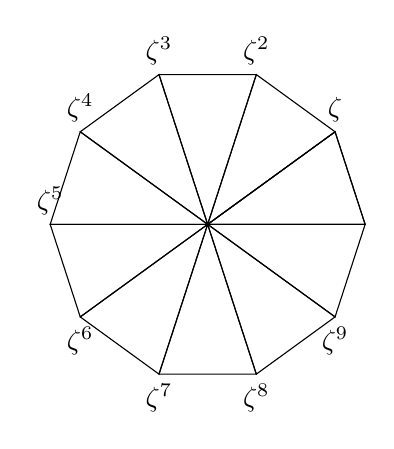
\begin{tikzpicture}[scale=2]
  \draw (0,0) -- (1,0) -- (36:1) -- cycle; 
  \draw (36:1) node[above] {$\zeta$};
  \draw (72:1) node[above] {$\zeta^2$};
  \draw (108:1) node[above] {$\zeta^3$};
  \draw (144:1) node[above] {$\zeta^4$};
  \draw (180:1) node[above] {$\zeta^5$};
  \draw (216:1) node[below] {$\zeta^6$};
  \draw (252:1) node[below] {$\zeta^7$};
  \draw (288:1) node[below] {$\zeta^8$};
  \draw (324:1) node[below] {$\zeta^9$};
  \begin{scope}[rotate=36]
   \draw (0,0) -- (1,0) -- (36:1) -- cycle;  
  \end{scope}
  \begin{scope}[rotate=72]
   \draw (0,0) -- (1,0) -- (36:1) -- cycle;  
  \end{scope}
  \begin{scope}[rotate=108]
   \draw (0,0) -- (1,0) -- (36:1) -- cycle;  
  \end{scope}
  \begin{scope}[rotate=144]
   \draw (0,0) -- (1,0) -- (36:1) -- cycle;  
  \end{scope}
  \begin{scope}[rotate=180]
   \draw (0,0) -- (1,0) -- (36:1) -- cycle;  
  \end{scope}
  \begin{scope}[rotate=216]
   \draw (0,0) -- (1,0) -- (36:1) -- cycle;  
  \end{scope}
  \begin{scope}[rotate=252]
   \draw (0,0) -- (1,0) -- (36:1) -- cycle;  
  \end{scope}
  \begin{scope}[rotate=288]
   \draw (0,0) -- (1,0) -- (36:1) -- cycle;  
  \end{scope}
  \begin{scope}[rotate=324]
   \draw (0,0) -- (1,0) -- (36:1) -- cycle;  
  \end{scope}
  \begin{scope}[rotate=360]
   \draw (0,0) -- (1,0) -- (36:1) -- cycle;  
  \end{scope}
 \end{tikzpicture}
\caption{各タイルの頂点座標}
\end{figure}
\begin{itemize}
 \item [拡大]
複素平面上の全体を$\tau$倍する操作である。$\tau=\zeta+\zeta^{-1}$
なので、$x=(x_0,x_1,x_2,x_3,x_4)$とすると、
\begin{equation}
 \tau x =(x_1-x_4, x_0+x_2, x_1+x_3, x_2+x_4, x_3-x_0)
\end{equation}
と表せる。

 \item [細分]
複素数xとyが与えられた時、それに対応する$5$次元座標を$x=(x_0,x_1,....,x_4)$,
$y=(y_0,y_1,...,y_4)$とすると、細分$x-y$を$\tau:1$に内分する点は
\begin{equation}
 \frac{x+\tau y}{\tau+1}
\end{equation}
と表せる。
\item [拡大後の細分]
xとyを$\tau$倍した点$\tau x$と$\tau y$を$\tau:1$に内分する。
\[
 \frac{(\tau x)+\tau(\tau y)}{\tau+1}
\]
である。$\tau^2=\tau+1$を用いると
\[
 \frac{(\tau x)+\tau(\tau y)}{\tau^2}=\frac{1}{\tau}x+y
\]
と変形できる。式(2.2)より
\[
 \frac{1}{\tau} x+y=(\tau-1)x+y
=\tau x-x+y
\]

\end{itemize}
式(2.4)を代入すると
\[
 (x_1-x_4, x_0+x_2, x_1+x_3, x_2+x_4, x_3-x_0)-x+y
\]
と表せる。

タイプAのタイルに拡大細分を2度施すと以下のようになる。
\begin{figure}[H]
  \begin{tikzpicture}[scale=2.5]
   \draw (0,0) -- (1,0) -- (36:1) -- cycle;
   \begin{scope}[scale=(sqrt(5)+1)/2,xshift=0.8cm]
    \draw (0,0) -- (1,0) -- (36:1) -- cycle; 
    \draw ({(sqrt(5)-1)/2},0) -- (36:1) --(1,0) -- cycle;
   \end{scope}
   \begin{scope}[scale=(sqrt(5)+1)/2+1,xshift=1.2cm]
    \draw (0,0) -- (1,0) -- (36:1) -- cycle; 
    \draw ({(sqrt(5)-1)/2},0) -- (36:1) --(1,0) -- cycle;  
   \end{scope}
   
   
 \end{tikzpicture} 
\end{figure}


 
\chapter{ライツアウト}
\section{構成法}

\end{document}
